%%%%%%%%%%%%%%%%%%%%%%%%%%%%%%%%%%%%%%%%%
% Beamer Presentation
% LaTeX Template
% Version 1.0 (10/11/12)
%
% This template has been downloaded from:
% http://www.LaTeXTemplates.com
%
% License:
% CC BY-NC-SA 3.0 (http://creativecommons.org/licenses/by-nc-sa/3.0/)
%
%%%%%%%%%%%%%%%%%%%%%%%%%%%%%%%%%%%%%%%%%

%----------------------------------------------------------------------------------------
%	PACKAGES AND THEMES
%----------------------------------------------------------------------------------------

\documentclass{beamer}
\usepackage{amssymb}
\usepackage{mathpazo}

\mode<presentation> {

% The Beamer class comes with a number of default slide themes
% which change the colors and layouts of slides. Below this is a list
% of all the themes, uncomment each in turn to see what they look like.

%\usetheme{default}
%\usetheme{AnnArbor}
%\usetheme{Antibes}
%\usetheme{Bergen}
%\usetheme{Berkeley}
%\usetheme{Berlin}
\usetheme{Boadilla}
%\usetheme{CambridgeUS}
%\usetheme{Copenhagen}
%\usetheme{Darmstadt}
%\usetheme{Dresden}
%\usetheme{Frankfurt}
%\usetheme{Goettingen}
%\usetheme{Hannover}
%\usetheme{Ilmenau}
%\usetheme{JuanLesPins}
%\usetheme{Luebeck}
%\usetheme{Madrid}
%\usetheme{Malmoe}
%\usetheme{Marburg}
%\usetheme{Montpellier}
%\usetheme{PaloAlto}
%\usetheme{Pittsburgh}
%\usetheme{Rochester}
%\usetheme{Singapore}
%\usetheme{Szeged}
%\usetheme{Warsaw}

% As well as themes, the Beamer class has a number of color themes
% for any slide theme. Uncomment each of these in turn to see how it
% changes the colors of your current slide theme.

%\usecolortheme{albatross}
%\usecolortheme{beaver}
%\usecolortheme{beetle}
%\usecolortheme{crane}
%\usecolortheme{dolphin}
%\usecolortheme{dove}
%\usecolortheme{fly}
%\usecolortheme{lily}
%\usecolortheme{orchid}
%\usecolortheme{rose}
%\usecolortheme{seagull}
%\usecolortheme{seahorse}
%\usecolortheme{whale}
%\usecolortheme{wolverine}

%\setbeamertemplate{footline} % To remove the footer line in all slides uncomment this line
%\setbeamertemplate{footline}[page number] % To replace the footer line in all slides with a simple slide count uncomment this line

%\setbeamertemplate{navigation symbols}{} % To remove the navigation symbols from the bottom of all slides uncomment this line
}
\def\Xint#1{\mathchoice
{\XXint\displaystyle\textstyle{#1}}%
{\XXint\textstyle\scriptstyle{#1}}%
{\XXint\scriptstyle\scriptscriptstyle{#1}}%
{\XXint\scriptscriptstyle\scriptscriptstyle{#1}}%
\!\int}
\def\XXint#1#2#3{{\setbox0=\hbox{$#1{#2#3}{\int}$ }
\vcenter{\hbox{$#2#3$ }}\kern-.6\wd0}}
\def\ddashint{\Xint=}
\def\dashint{\Xint-}
\usepackage{graphicx} % Allows including images
\usepackage{booktabs} % Allows the use of \toprule, \midrule and \bottomrule in tables
\mode<presentation>{}
%----------------------------------------------------------------------------------------
%	TITLE PAGE
%----------------------------------------------------------------------------------------

\title[prediction and learning]{On PDE approach to some machine learning problems} % The short title appears at the bottom of every slide, the full title is only on the title page

\author{Hong Zhang} % Your name
\institute[Brown University] % Your institution as it will appear on the bottom of every slide, may be shorthand to save space
{
Applied Math, Brown University \\ % Your institution for the title page
\medskip
}
\date{\today} % Date, can be changed to a custom date

\begin{document}

\begin{frame}
\titlepage
\end{frame}
\begin{frame}
\tableofcontents
\end{frame}

\section{Introduction}

\begin{frame}
Partial differential equations (PDEs) are used to describe many phenomenons.  Many famous PDEs are from physics.
\begin{itemize}
\item Heat: heat equation, $u$ tempature
\begin{columns}
\column{0.6\textwidth}
\begin{equation*}
\partial_t u = \sum_{i=1}^3\frac{\partial^2 u }{\partial x_i^2} = \Delta u
\end{equation*}
\column{0.4\textwidth}
\begin{figure}
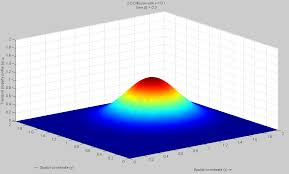
\includegraphics[scale = 0.3]{heatdiffusion}
%\caption{Viscous flow}
\end{figure}
\end{columns}
\pause
\item Fluid mechanics: Naiver-Stokes equation
\begin{columns}
\column{0.6\textwidth}
\begin{align*}
\partial_t u + (u\cdot\nabla)u - \Delta u = -\nabla p.
\end{align*}
\column{0.4\textwidth}
\begin{figure}
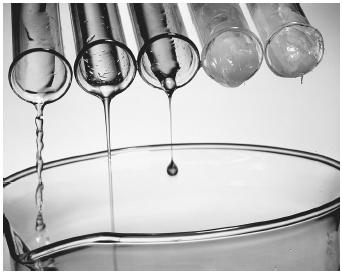
\includegraphics[scale = 0.25]{viscosflow}
%\caption{Viscous flow}
\end{figure}
\end{columns}
\pause
\item Quantum mechanics, electrodynamics, image processing,\ldots.
\end{itemize} 


\end{frame}

\begin{frame}
\frametitle{Probability and PDEs}
\begin{columns}
\column{0.5\textwidth}
\begin{figure}
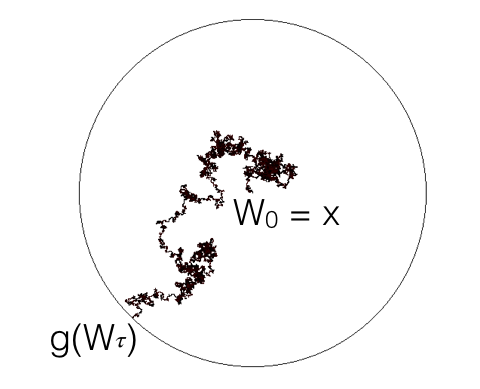
\includegraphics[scale = 0.3]{bmotion.png}
\caption{Brownian Motion}
\end{figure}
\column{0.5\textwidth}
$W_t$: a Brownian motion with $W_0 = x$. $W$ hits boundary at $W_{\tau}$.  $u(x) = \mathbb{E}^x[g(W_\tau)]$.
Then $$\Delta u = 0,$$ 
and $$u = g\quad \text{on}\quad S_1.$$


\end{columns}
\end{frame}

\begin{frame}
\frametitle{Online Learning: Examples}

\begin{columns}
\column{0.5 \textwidth}
\begin{figure}

\includegraphics[scale = 0.4]{spam}
\caption{Spam Detection}
\end{figure}
\column{0.5\textwidth}
\begin{itemize}
\item emails arrive one by one
\pause
\item spam detector makes prediction for each of them: {\color{blue}spam or not}
\pause
\item sometimes get {\color{blue}feedback} from users
\pause
\item make better detection next time  
\end{itemize}

\end{columns}

\end{frame}

\begin{frame}
\frametitle{Online Learning: Example 2}
\begin{columns}
\column{0.5 \textwidth}
\begin{figure}

\includegraphics[scale = 0.4]{recommendation}
\caption{Recommendation}
\end{figure}
\column{0.5\textwidth}
\begin{itemize}
\item users visit Netflix /Amazon/\ldots
\pause
\item movies/products/\ldots are recommended 
\pause
\item users {\color{blue}click or not}
\pause
\item make better recommendation next time   
\end{itemize}

\end{columns}


\end{frame}

\begin{frame}
\frametitle{Why Online Learning?}
\begin{itemize}
\item Batch learning:
\begin{itemize}
\item distribution fixed over time (training and test)
\item i.i.d. assumptions
\item a fixed predictor 
\end{itemize}
\pause
\item Online learning:
\begin{itemize}
\item no distribution assumption
\item suitable for changing or adversarial environment  
\item a natural model for many applications, mixing training and test 
\item memory efficient
\end{itemize}
\end{itemize}
\end{frame}




\section{Prediction with Expert Advice}
\begin{frame}
\frametitle{Prediction With Expert Advices}
\begin{itemize}
\item Need: to make a decision every day
\begin{columns}
\column{0.7\textwidth}
	\begin{itemize}
	\item which stock to invest in
	\item which route to drive home
	\item \ldots
	\end{itemize}
\column{0.3\textwidth}
\begin{figure}

\includegraphics[scale = 0.25]{question}
%\caption{Viscous flow}
\end{figure}
\end{columns}
\pause
\item Given: advice from a set of experts
	\begin{columns}
	\column{0.7\textwidth}
	\begin{itemize}
	\item financial adviser
	\item Route 1, Route I-95, Route 295,\ldots
	\item \ldots
	\end{itemize}
	\column{0.3\textwidth}
	\begin{figure}

\includegraphics[scale = 0.25]{experts}
%\caption{Viscous flow}
\end{figure}
\end{columns}
\pause	
\item Question:
	\underline{How to combine advice and make smart choices?}
\end{itemize}

\end{frame}


\subsection{A simple example}
\begin{frame}
\frametitle{Gentle Start: a simple example}
\begin{itemize}
\item Set up:
\begin{itemize}
\item Predict an unknown sequence $y_1, y_2, \ldots,$ where $y_i\in\{0,1\}.$
\pause
\item $N$ experts provide advice $(f_{1,t},f_{2,t},\ldots, f_{N,t})$
\pause
\item A forecaster makes her guess $\hat{p}_t\in\{0,1\}$ for $y_t$ 
\pause
\item True $y_t$ is revealed and find if $\hat{p}_t = y_t$. 
\pause
\item Know that one of the experts makes no mistakes.
\pause
\end{itemize}
\item Goal: bound the number of the mistakes made by the forescaster
\end{itemize}
\end{frame}

\begin{frame}
\frametitle{Halving Algorithm}
{\bf Algorithm:}
\begin{itemize}
\item at time $t$, expert $i$ has weight $w_i^t$
\pause
\item originally, $w_i^0 = 1, \forall i\in[1,N]$
\pause
\item prediction according to the weighted majority 
\pause
\item update each wrong expert   $w_i^t = 0$
\pause
\end{itemize}
{\bf Conclusion}: the number of mistakes made by the forecaster is bounded by {\color{red}$\lfloor\log_2 N\rfloor$}.
\end{frame}

\begin{frame}
\frametitle{Proof}:
\begin{itemize}
\item let $w_m$ be the sum of the weight of all experts after the forecaster has made $m$ mistakes.
\pause
\item Initially, $w_0 = N.$
\pause
\item When the forecaster make her $m$th mistakes, at least half of the experts have been always correct make their first mistake
\begin{equation*}
w_m \le \frac{w_{m-1}}{2}\Longrightarrow w_m\le \frac{w_0}{2^m}.
\end{equation*} 
\pause
\item $w_i =1$  for some $i$
\begin{equation*}
m\le \lfloor\log_2 N\rfloor.
\end{equation*}
\end{itemize}


\end{frame}
\begin{frame}
\frametitle{More general setting:}
\begin{itemize}
\item Do not know there is one expert who makes no mistakes. 
\pause
\item Weighted Majority Algorithm:
\begin{itemize}
	\item at any time, expert $i$ has weight $w_i^t$.
	\item originally, $w_i^t = 1, \forall i\in[1,N]$.
	\item prediction according to weighted majority. 
	\item weight of each wrong expert updated ($\beta\in(0,1)$)
	$$w_i^{t+1}\leftarrow w_i^t\beta.$$
\end{itemize}
\pause
\item Theorem: let $m_i^t$ be the number of mistakes made by expert $i$ till time $t$ and $m^t$ be the number of mistakes made by the WM algorithm. Then
$$m_t \le \frac{\log_2 N+m_i^t\log_2\frac{1}{\beta}}{\log_2 \frac{2}{1+\beta}}.$$
\begin{itemize}
\item $m_t\le O(\log_2 N)+\text{constant}\times\text{best expert}$.
\end{itemize}

\end{itemize}
\end{frame}


\begin{frame}
\frametitle{Remarks:}
\begin{itemize}
\item Linear dependence on the best expert
\pause
\item Independent of the number of predictions
\pause
\item Independent of the choice of sequence of outcomes
\pause
\item Mild dependence on the number of the experts
\end{itemize}


\end{frame}







\begin{frame}
\frametitle{General Setting}
\begin{itemize}
\item{For $t = 1$ to $T$ do}
	\begin{itemize}
	\item{receive instance $x_t\in X$ and advice $\hat{y}_{t,i}\in Y$, $i\in [1,N]$}
	\item{predict $\hat{y}_t\in Y$}
	\item{receive label $y_t\in Y$}
	\item{incur loss $L(y_t,\hat{y}_t)$}
	\end{itemize}
\pause
\item {\color{red}Objective:} minimize regret, i.e., difference of total loss incurred and that of best exeprt:
$$Regret(T) = \sum_{t=1}^TL(y_t,\hat{y}_t)-\min_{i\in[1,N]}\sum_{t=1}^TL(y_t,\hat{y}_{t,i}).$$
\pause	
\item Goal: obtain {\color{red}sublinear regret} to the {\color{red}best expert}. (top 10 experts, any competitor, etc. )
$$\lim_{T\to \infty}\frac{Regret(T)}{T} = 0.$$
\end{itemize}


\end{frame}

\begin{frame}
\frametitle{An Optimal Bound}
\begin{itemize}
\item Exponential weighted average

\begin{itemize}
\item weight update:
$$w_i^{t+1} \leftarrow w_i^t e^{-\eta_t L_{t,i}},$$
where $L_{t,i}$ is total loss incurred by expert $i$ till time $t$
\item prediction:
$$\hat{y_t} = \frac{\sum_{i=1}^Nw_{i}^ty_{t,i}}{\sum_{i=1}^Nw_{i}^t}.$$ 
\end{itemize}
\pause
\item Theorem: Assume $L$ is convex in its first argument and takes values in $[0,1]$. Then for any $T$
$$Regret(T)\le \frac{\sqrt{2}}{\sqrt{2}-1}\sqrt{(T/2)\log_2 N}+\sqrt{\log_2 N/2}.$$


\end{itemize}


\end{frame}
\begin{frame}
\frametitle{Remarks on the theorem}
\begin{itemize}
\item When the loss is between $[0,1]$ 
$$Regret(T) = O(\sqrt{(\log N) T}).$$
\pause
\item The bound can be improved if more information is known, e.g., if the loss functions are special, $L_2$ loss, $L_1$ loss, 
\pause
\item In general, the bound is asymptotically optimal. 

\end{itemize}


\end{frame}



\begin{frame}
\frametitle{Active research area: literatures}
\begin{itemize}
\item Littlestone and Warmuth develop {\color{blue}weighted majority algorithm}
\item Cesa-Bianchi et al. obtain minimax regret bounded by $\sqrt{(T/2)\log N}.$
\item Cesa-Bianchi and Lugosi connected the regret with the Rademacher Complexity of the set of experts.
\item Even-Dar et al. considered regret to the average

\item Rakhlin et al. developed {\color{blue}Sequential Rademacher Complexity} to study online learning.
\item \ldots
\end{itemize}


\end{frame}



\subsection{PDE approach of prediction problem}

\begin{frame}
\frametitle{A naive prediction problem (T.Cover, 1965)}
\begin{itemize}
\item Predict $y_1,y_2,\ldots$, where $y_t\in\{-1,1\}$ ({\color{blue}stock goes up or down}). 
\pause
\item Forecaster makes prediction $\hat{p}_t\in[-1,1]$ ({\color{blue}buy/sell $\hat{p}_1$ shares of stocks}) according to some algorithm $\hat{P}$. 
\pause
\item At each time $t$, investor loss (or gain) $-\hat{p}_ty_t$. Cumulative loss (or gain)
$$L(\hat{P},y_T) := -\sum_{t=1}^T\hat{p}_ty_t$$
\pause
\item Two naive experts: one always predicts 1 ({\color{blue}always goes up}); the other one always predicts -1({\color{blue}always goes down}).
\end{itemize}
Cover proved $$Regret(T) = \Theta(\sqrt{T}).$$

\end{frame}

\begin{frame}
\frametitle{PDE approach}
This problem was considered by Kohn using PDE technique.  
\begin{itemize}
\item Instead of proposing an algorithm and then proving the asymptotic bound, PDE method focuses on the optimal strategy
\pause
\item Typical Goal: minimize the worst-case regret with respect to the best performing expert.
\pause
\item More general goal: minimize the worst case value of 
$$\phi(\text{regret with respect to expert ``1'', regret with respect to expert ``-1''})$$
at time $T$. (``Typical goal'' is $\phi(x_1,x_2) = \max\{x_1,x_2\}$.)
\end{itemize}


\end{frame}

\begin{frame}
\frametitle{Two very simple experts}
Essentially,  the problem is an optimal control problem:
\begin{itemize}
\pause
\item{\color{red}state space:}$$(x_1,x_2) = (\text{regret w.r.t.  expert ``1'', regret w.r.t.  expert ``-1''}).$$
\pause
\item {\color{red}control:} prediction $\hat{p}_t\in[-1,1]$ ({\color{blue}investor's purchase bounded by 1}) 
\pause
\item {\color{red}value function:} $v(x,t) = $ optimal time $T$ result, starting from relative regrets $x = (x_1,x_2)$ at time $t$. 
\end{itemize}

{\color{red}Dynamical programming principle:}
\begin{align*}
v(x_1,x_2,t) &= \min_{|p|\le 1}\max_{b = \pm 1}v(\text{new position},t+1)\\
                    & = \min_{|p|\le 1}\max_{b = \pm 1}v(x_1 + b(1-p),x_2-b(1+p),t+1)		
\end{align*}
for $t<T$, with final-time condition $v(x,T) = \phi(x).$

\end{frame}

\begin{frame}
\frametitle{Dynamical Programming Principle}
Recall: {\color{red}$(x_1,x_2) = (\text{regret w.r.t. ``'1'' expert, regret w.r.t. ``-1'' expert})$}, where regret  = (investor's loss) - (expert's loss).
\vfill
If the investor buys $p$ shares and the market goes up, investor loss $-p$, the 
``+'' expert loss $-1$, the ``-1'' expert loss $1$. So the state moves from $(x_1,x_2)$ to $(x_1-(1-{p}),x_2+(1+{p})).$
\vfill
Similarly, if investor buys ${p}$ shares  and market goes down, state move from $(x_1,x_2)$ to $(x_1+(1-{p}),x_2-(1+{p})).$
\vfill
Hence the dynamical programming principle:
 \begin{align*}
 v(x_1,x_2,t) = \min_{|p|\le 1}\max_{b = \pm 1}v(x_1 + b(1-p),x_2-b(1+p),t+1).
 \end{align*}

\end{frame}

\begin{frame}
\begin{itemize}
\item Want to know how the regret accumulates as $T\to \infty$.
\pause
\item To access this question, it is natural to rescale the problem and look for a continuum limit.
\pause
\item Our scaling is like the passage from random walk to Brownian motion.
 \begin{itemize}
 \item Let $\xi_1,\xi_2,\ldots$ be i.i.d. random variable with mean 0 and variance 1. For each $n$, define a continuous-time stochastic processes $\{W_n(t)\}$
 $$W_n(t) = \frac{1}{\sqrt{n}}\sum_{1\le j\le [nt]}\xi_j.$$ 
Then $W_n(t)\to W_t,$ where $W_t$ is a standard Brownian motion.
\end{itemize}

\end{itemize}

\end{frame}

\begin{frame}
\begin{itemize}
\item So we consider a {\color{red}scaled} version of the problem: stock moves {\color{red}$\pm \epsilon$}, time steps are {\color{red}$ \epsilon^2$}, and the scaling of regret is ${\color{red}\epsilon^2}$. The value function is still the optimal time-T result.  The dynamical programming principle becomes
\begin{align*}
w^\epsilon(x_1,x_2,t) = \min_{|p|\le 1}\max_{b = \pm 1} w^\epsilon(x_1 + \epsilon b(1-p),x_2-\epsilon b(1+p),t+\epsilon^2)
\end{align*}
\pause
\item We expect as $\epsilon\to 0$, $w^\epsilon(x,t)\to w(x,t)$ and $w$ solves some PDEs.
\end{itemize}

\end{frame}

\begin{frame}
\title{PDE}
The partial differential equation is the {\color{red}Hamilton-Jacobi-Bellman} equation associate with the optimal control problem.  Formal derivation 
\begin{enumerate}
	\item Use the Taylor's expansion to estimate
	$$w(x_1+\epsilon b(1-p),x_2-\epsilon(1+p),t+\epsilon^2).$$
	\item Investor choose $p$ to make $O(\epsilon)$ terms vanishes; this gives 
	$$p = \frac{\partial_1 w - \partial_2 w}{\partial_1 w + \partial_2 w}. ({\color{red}\text{optimal strategy}})$$ 
	\item The $O(\epsilon^2)$ are insensitive to $b = \pm 1$; they give the nonlinear PDE
	$$w_t + 2<D^2 w \frac{\nabla^\perp w}{\partial_1 w + \partial_2 w},\frac{\nabla^\perp w}{\partial_1 w+\partial_2 w}> = 0,$$
	where $\nabla^\perp w = (\partial_2 w,-\partial_1 w).$ Prescribe the final value $w = \phi$ at $T$.
\end{enumerate}
\end{frame}
%\begin{frame}
%\frametitle{More detailed derivation of the PDE}
%Dynamical programming principle:
%$$w^\epsilon(x_1,x_2,t) = \min_{|p|\le 1}\max_{b = \pm 1} w^\epsilon(x_1 + \epsilon b(1-p),x_2-\epsilon b(1+p),t+\epsilon^2)$$
%Taylor's expansion:
%\begin{align*}
%&w(x_1 + \epsilon b(1-p),x_2-\epsilon b(1+p),t+\epsilon^2) \\
%&= w(x_1,x_2,t) + \epsilon b(1-p)\partial_1w -\epsilon b(1+p)\partial_2 w+ \partial_t w\epsilon^2 \\
%&+\frac{1}{2}\partial_{11}w\epsilon^2 b^2(1-p)^2-\partial_{12}w\epsilon^2 b^2(1+p)(1-p)+\frac{1}{2} \partial_{22}w\epsilon^2b^2(1+p)^2.
%\end{align*}
%\end{frame}

%\begin{frame}
%After substitution and reorganization:
%\begin{align*}
%&0\approx \max_{|p|\le 1}\min_{b = \pm 1}\{\epsilon b[(1-p)\partial_1 w-(1+p)\partial_2 w]\\
%&\epsilon^2 b^2 [\frac{1}{2}\partial_{11}w(1-p)^2 -\partial_{12}w(1-p)(1+p) + \frac{1}{2}\partial_{22}w(1+p)^2 + \partial_t w]\}
%\end{align*}
%$O(\epsilon)$ terms vanishes and obtain
%\begin{align*}
%p = \frac{\partial_1 w-\partial_2 w}{\partial_1w +\partial_2 w}.
%\end{align*}
%Note: we expect $\partial_1 w >0$ and $\partial_2 w>0$, which implies $|p|\le 1$. 
%
%\end{frame}

\begin{frame}
\frametitle{Conclusion}
%Under some assumptions on the terminal data $\phi$, we can show that
%\begin{itemize}
%\item solution exists under very general conditions on $\phi$
%\item $w$ is pretty regular or $C^k$ for some $k\ge 0$ 
%\item $|\nabla w|\neq 0$
%\item $w_t<0$
%\end{itemize}
%Convergence result:
\begin{itemize}
\item if $\phi$ smooth
\begin{align*}
\|w^\epsilon(x,t)-w(x,t)\|\le C\epsilon,
\end{align*}
where $C$ independent of $t$.
\item if $\phi(x) = \max\{x_1,x_2\}$
\begin{align*}
\|w^\epsilon(x,t)-w(x,t)\|\le C\epsilon\log\epsilon.
\end{align*} 
\item Equation can be solved explicitly.
\end{itemize}
\end{frame}

%\begin{frame}
%\frametitle{Application of the theory} 
%Consider the terminal time is $t = 0$ and the equation is satisfied in $(-\infty,0)\times \mathbb{R}^2$. Make an anstaz:
%\begin{align*}
%w(t,x,y) = \frac{x+y}{2}-\sqrt{-t}g(\frac{x-y}{\sqrt{-t}}).
%\end{align*}
%Then $g$ satisfies a Hermite ODE
%\begin{align*}
%g(z) - zg'(z) - 16g''(z)= 0,
%\end{align*}
%which can be solved explicitly.
%\vfill
%The optimal strategy 
%$$
%f = -2g'(\frac{x-y}{\sqrt{-t}}).
%$$
%\end{frame}


\begin{frame}
\frametitle{Discussion}
\begin{itemize}
\item Stock prediction problem has a continuous-time limit. The PDE has a rather explicit solution. 
\pause
\item Problem is considered as a deterministic two-person game.
\pause
\item One can consider more complex situation, e.g., more experts, more intelligent experts, etc.
\pause
\item Dynamical programming principle can be hard to derive.
\end{itemize}
\end{frame}





\section{Stochastic Control}


\begin{frame}{Reinforcement Learning}
\begin{figure}
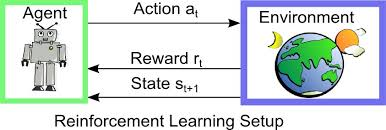
\includegraphics[scale = 0.5]{reinforcementlearning}
\end{figure}
S: Set of states

A: Set of actions

R: Reward function. $\forall s_t,a_t$, $r_t = R(s_t,a_t)\in \mathbb{R}$

  
\end{frame}


\begin{frame}
\begin{itemize}
\item In the previous example, we derive the PDE from {\color{red}Hamilton-Jacobi-Bellman} equation of a optimal control problem. 
\pause
\item In the discrete case, Markov decision process (MDP) is a discrete time stochastic control process. (Reinforcement Learning).   The value function $v:S\to \mathbb{R}$ satisfies a discrete Bellman equation.
\pause
\begin{itemize}
\item Given a policy $\pi$ with infinite horizon for any state $x\in X$
\begin{equation*}
V_\pi(x) = R(x,\pi(x)) + \gamma\sum_{x'\in X}P(x'|x,\pi(x))V_{\pi}(x')
\end{equation*}
\item Optimal policy
\begin{align*}
V^\ast(x) = \max_{a\in A}\{R(x,a) + \gamma\sum_{x'\in X}P(x'|x,a)V_{\pi}(x')\}
\end{align*}
\end{itemize}

\end{itemize} 
\end{frame}

\begin{frame}
\begin{itemize}
\item Continuous time and state: PDEs. 
\begin{itemize}
\item Dynamics of the state
\begin{align}\label{eq1}
dX_s = b(X_s,a_s)\,ds + \sigma(X_s,a_s)\,dW_s,
\end{align}
where $W_s$ is Brownian motion and $a_s$ is control process.
\pause
\item Reward 
\begin{align*}
R(t,x,a) = \mathbb{E}\big[\int_t^Tf(X_s^{t,x},a_s)\,ds + g(X_T^{t,x})\big],
\end{align*}
where $X^{t,x}$ is the solution of \eqref{eq1} starting from $X_t = x$.
\pause
\item Value function 
$$v(t,x) = \sup_{a\in \mathcal{A}}R(t,x,a).$$
\pause
\item HJB equation 
$$\frac{\partial v}{\partial t} + \sup_{a\in \mathcal{A}}(L_a v + f(x,a)) = 0\quad \text{in} [0,T]\times \mathbb{R}^d,$$
where $L_a$ is the infinitesimal generator of the process \eqref{eq1}. 
\end{itemize}
\end{itemize}

\end{frame}

\section{Elliptic PDEs}
\begin{frame}
\frametitle{Second-order Linear Elliptic PDEs}
A classical example is 
\begin{equation*}
\Delta u(x) = \sum_{i=1}^d\frac{\partial^2 u}{\partial x_i^2}= 0.
\end{equation*}
Let $W_t$ be a Brownian motion starting from $x$. Then 
\begin{align*}
\lim_{t\to 0}\frac{E^xu(W_t)-u(x)}{t} = \frac{1}{2}\Delta u.%\quad  (\text{by It\^{o}'s formula}). 
\end{align*}
General diffusion process
$$L_a u = \frac{1}{2}Tr(\sigma \sigma^T D^2 u) = \frac{1}{2}\sum_{i,j=1}^da_{ij}D_{ij}u,$$ 
where $\{a_{ij}\}$ is some positive-definite matrix.

\end{frame}
\begin{frame}
\frametitle{HJB equation}
Fully nonlinear equation ({\color{red}$v$ depends on $(t,x)$})
\begin{equation*}
{\color{red}\partial_t v} + \sup_{a\in \mathcal{A}}(L_a v +f(x,a)) = 0,
\end{equation*}
where $L_a$ is a second-order linear elliptic operator. 

\vfill
After deriving the HJB equation formally,  the equation holds in a weak sense. The regularity of the solution is very low. 
\begin{itemize}
\item Easy to find solution in the space of continuous function 
\item Equation holds in a very weak sense (viscosity solution).
\item Important problem in the PDE community to prove the existence of classical solution.
\end{itemize}
\end{frame}

\begin{frame}

\frametitle{Mathematical Result}
Recall:
$$
dX_s = b(X_s,a_s)\,ds + \sigma(X_s,a_s)\,dW_s.
$$

Under some regularity assumption on the coefficients $\sigma,b$, then the solution to the HJB
$$
{\partial_t u} + \sup_{a\in \mathcal{A}}(L_a u +f(x,a)) = 0,
$$
is a classical solution. Rigorously, $u\in C^{2,\alpha}$ for some $\alpha>0$. 
\vfill
The theoretical results helps to build numerical scheme to solve the HJB.
\end{frame}

\begin{frame}
\frametitle{Jump processes and Nonlocal equations}
Brownian motion is a continuous stochastic process. Consider more general process: L\'evy processes (jump processes)
$$dX_s = b(X_s,a_s)\,ds + \sigma(X_s,a_s)\,dY_s,$$
where $Y_s$ is a L\'evy process. The infinitesimal generator of such processes is nonlocal 
$$
L_a u = \int_{\mathbb{R}^d}(u(x+y)+u(x-y)-2u(x))\frac{K_a(y)}{|y|^{d+\sigma}}\,dy,
$$ 
and $\sigma\in(0,2).$
\end{frame}


\begin{frame}
\begin{theorem}
Let $v$ be a weak solution to 
\begin{equation*}
v_t + \sup_a (L_av + f_a) = 0,
\end{equation*}
where $L_a$ is a nonlocal operator defined previously. Then the solution $v$ is a classical solution and derivatives of $v$ are bounded.
\end{theorem}
\end{frame}

\begin{frame}
\center
\huge Thank you.

\end{frame}




\end{document}